\chapter{Modeling users' behaviors}\label{sec:users-behaviors}

    If we want to infer some information about a huge graph, such as the ones behind the web or Facebook, we usually can't perform our computation directly on the real graph, so we use models of the graph.

    Some properties we usually are interested in when dealing with a network (or a graph) are the following:
    \begin{itemize}
        \item the overall number of nodes,
        \item the average degree,
        \item the number of nodes with a certain degree,
        \item the size of the communities,
        \item the degree distribution.
    \end{itemize}


\section{Erdős–Rényi model}\label{sec:gnp}
    
    This is a model for generating random graph, that has many applications due to its simplicity, but doesn't fit real world networks: each node has more or less the same degree, based on a fixed probability, while real networks have a gaussian distribution of the degrees.
    
    We denote by $G(n, p)$ a random process that produces a graph with $n$ nodes, in which each edge appears with probability $p$. This process can be described by the following algorithm:
    \begin{lstlisting}[caption={The G(n,p) algorithm},label={lst:gnp}]
Sample G(n,p):
    let $E := [n]$
    $E \gets \emptyset$
    for each $\{i, j\} \in \binom{V}{2}$:
        flip a coin with head probability $p$
        if the coin comes up head:
            $E \gets E \cup \{\{i,j\}\}$
    return $G(V,E)$
    \end{lstlisting}
    
    We are interested in studying the properties oh the graphs generated by this process when the parameter $p$ changes.
    

\subsection{Degree distribution}\label{sec:gnp-degree}

    We begin our study of $G(n,p)$ graphs looking at their degree distribution.
    
    \begin{obs}
        The average degree of each node in $G$ is:
        \begin{flalign}\label{eq:gnp-deg}
            &\mathbb{E}[\deg(i)] = \sum_{j \neq i} \Pr{ \{i, j\} \in E } = \sum_{j \neq i} p = (n-1)p&
        \end{flalign}
    \end{obs}

    At this point we aren't sure if this information is valuable, since it could be that the actual degrees are far from the average (i.e. there is high variance), so we want to proof that, instead, those values are \textit{concentrated} around the average.\\
    Let $X = \deg(i) = \sum_{j \neq i} x_j$ where $x_j =
    \begin{cases}
   		1 & \text{if } \{i,j\} \in E(G) \text{ \ \ \ \ (with probability } p)\\
        0 & \text{otherwise} \text{ \ \ \ \ (with probability } 1-p)\\
    \end{cases}$ \\
    and the $x_j$ are mutually independent.
    
    Thanks to the mutual independence of the $x_j$, we can apply the Chernoff Bound [\ref{chernoff}] to prove our claim:
    \begin{flalign*}
        &X = \sum x_j = \frac{n}{2} \pm \sqrt{n \ln \frac{1}{\delta}} \text{ with probability } 1 - O(\delta)&
    \end{flalign*}
    
    Thus, since in average each node has the same degree, $G(n,p)$ produces \textit{almost regular graphs}, that are not suitable for representing real world social graphs, as stated at the beginning of this section.
    

\subsection{Connectivity}\label{sec:gnp-connectivity}
    Now we want to analize with which probability $G(n,p)$ will produce a connected graph $G=(V,E)$.
    
    \begin{thm}[Connectivity of G(n,p)]\label{thm:gnp-connectivity}
        If $p \geq \frac{8 \ln n}{n}$, then $G(n,p)$ is connected with probability $\geq 1 - \frac{1}{n}$.
    \end{thm}

    Before going into the proof of the theorem, we introduce a combinatorial property that will be useful later.
    
    \begin{lem}\label{l:gnp-connectivity}
        If $\forall\ \emptyset \subset S \subset V,\ \exists \{u,v\} \in E$ such that $u\in S,\ v \in V-S$, then the graph is connected.
    \end{lem}

    \begin{figure}[h!]
        \centering
        \includegraphics[scale=0.5]{gnp_l1}
        \caption{inductive proof of the lemma}
        \label{fig:gnp-l1}
    \end{figure}

    \begin{proof}[Informal proof by induction] \
        \begin{itemize}
            \item Base step: In $S_0$ there is only the node $u_0$, so there must be an edge from $u_0$ to a node $v_1 \in V-S$;
            \item Inductive step: Go on expanding the frontier (the set of nodes in $S$ that have an edge connecting them to a node in $V-S$) until the BFS visit reaches all the nodes.
        \end{itemize}
    
        See the figure [\ref{fig:gnp-l1}].
    \end{proof}

    \begin{proof}[Proof of the theorem \ref{thm:gnp-connectivity}]
        Let $\xi_S$ be the bad event ``there are no edges in the cut ($S, V-S$)'' for each proper subset $S$ of $V$.
        
        Thanks to the lemma [\ref{l:gnp-connectivity}], we know that $\Pr{G(n,p) \text{ is not connected}} =
        \Pr{\bigcup_{S \subset V} \xi_S}$.
        
        Let's note that there are $2^n-2$ of such subsets, but we are interested only in half of the corresponding events, since $\xi_s = S_{V-S} \ \forall\ S \subset V$ (the events $\xi_i$ are \textbf{not} independent), so we will consider only the $\frac{1}{2}(2^n-2)$ events $\xi_S$ for which $|S| \leq \frac{|V|}{2}$.
        
        Let $n := |V|$ and $s := |S|$, now we can compute the probability of a single event $\xi_S$:
        \begin{flalign*}
            \Pr{\xi_S} &= (1-p)^{s \cdot (n - s)}&\tag{by [$*^1$]}\\
           &\leq e^{-p \cdot s \cdot (n - s)}&\tag{by [\ref{eq:e-x}]}\\
           &\leq e^{-p \cdot s \cdot n/2}&\tag{since $s \leq n/2$}\\
           &\leq e^{-\frac{8 \ln n}{n} \cdot s \cdot \frac{n}{2}}&\\
           &= \left( e^{-\ln n} \right)^{4 \cdot s} = n^{-4 \cdot s}&
        \end{flalign*}
        
        [$*^1$] there are $s \cdot |V-S|$ edges from $S$ to $V-S$, each of which does not appear w.p. $1-p$, and $s \cdot |V-S| = s \cdot (n - s)$.
        
        Now, let's consider the probability that $\xi_S$ happens for any $S \subset V$:
        \begin{flalign*}
            \Pr{\exists S \in \binom{V}{s} \st \xi_s \text{ happens}}
            &\leq \sum_{S \in \binom{V}{s}} \Pr{\xi_S}& \tag{by Union Bound [\ref{eq:union-bound}]}\\
            &\leq \sum_{S \in \binom{V}{s}} n^{-4s} = 
            \binom{n}{s} \cdot n^{-4s}&\tag{since $\abs{\binom{V}{s}} = \binom{n}{s}$}\\
            &\leq n^s \cdot n^{-4s} = n^{-3s}\tag{since $\binom{n}{s} \leq n^s$}&
        \end{flalign*}
        
        Now we are ready to compute the probability that $G$ is connected. To do that we will distribute sets in ``buckets'' according to their cardinality:
        \begin{flalign*}
            \Pr{G(n,p) \text{ is not connected}} &=
            \Pr{\bigcup_{S \subset V} \xi_S}&\\
            &= \Pr{\exists s \in \{1,\ldots, n\} \st \exists S \in \binom{V}{s} \st \xi_S \text{ happens}}&\\
            &\leq \sum_{s = 1}^{n/2} n^{-3s}&\tag{by Union Bound [\ref{eq:union-bound}]}\\
            &\leq \sum_{s = 1}^{n/2} n^{-3} = \frac{1}{2n^2}&
        \end{flalign*}
        
        So we proved that $\Pr{G(n,p) \text{ is connected}} 
        \geq 1 - \frac{1}{2n^2} \geq 1 - \frac{1}{n}$, so we showed a stronger claim than the one we wanted to prove.
    \end{proof}

    \begin{obs}
        The theorem we just proved is a so called \textit{zero-one law}: It holds for the given bound of $p$, but it ceases to hold almost immediately when $p$ goes under that bound, so $p = \frac{8 \ln n}{n}$ is sort of a threshold between $G(n,p)$s that produce connected graphs with high probability and $G(n,p)$s that produce \textbf{un}connected graphs with high probability.
    \end{obs}
    
     We won't proof exactly what we just claimed, since it would be hard, but something weaker:
    \begin{thm}
        If $p < \frac{\varepsilon}{n} \ll \frac{8 \ln n}{n}$, then $G(n,p)$ is disconnected with probability $\geq 1 - \varepsilon$.
    \end{thm}
    
    \begin{proof}
        Let $X := \deg(i)$ and $x_j$ defined as before (see [\ref{sec:gnp-degree}]).
        \begin{enumerate}
            \item $X = \sum_{j \neq i} x_j = \sum_{j \neq i} \Pr{\{ i,j \} \in E(G)}$;
            \item We know by hypothesis that $\mathbb{E}[X_j] = p < \frac{\varepsilon}{n}$;
            \item $\mathbb{E}[X] < (n-1) \frac{\varepsilon}{n}$;
            \item $\Pr{X \geq \frac{1}{\varepsilon} \cdot \mathbb{E}[X]} \leq \varepsilon$ (by Markov inequality [\ref{eq:markov2}]);
            \item Since $\frac{1}{\varepsilon} \cdot \mathbb{E}[X] \approx 1$ and $X$ has integer values, we can write the previous expression as \\
            $\Pr{X > 0} \leq \varepsilon$, and this is the probability that exists a node $i$ that has at least one neighbor;
            \item Thus, by complement, $\Pr{\exists\ i \st i \in V \text{ and } i \text{ has 0 neighbors}} = \Pr{G(n,p) \text{ is not connected}} \geq 1 - \varepsilon$.
        \end{enumerate}
    \end{proof}
    

\subsection{Diameter}
    It is known that with high probability $G(n,p)$ graphs have small diameter. The proof is left as an exercise.

    
\section{Preferential attachment}\label{sec:pref-att}
    
    This is another model for generating random graphs, but it follows the rule ``the rich get richer'', meaning that nodes with higher degree will see their degree becoming higher and higher.
    
    The rule used to build a graph is the following: when you have built a graph with $N-1$ nodes, you add the $N$-th node with an edge that goes from $N$ to a node $i$ chosen accordingly to the following probability:
    \begin{flalign*}
        &\Pr{\text{neighbor of $N$ is $i$}} = \frac{deg(i)}{\sum_{k=1}^{N} deg(k)}&
    \end{flalign*}
    where the denominator is a normalization factor.
    
    There exist many variants of this model, for example with each node creating $k$ edges instead of one, with no self-loop, etc.

    \begin{figure}[h!]
        \centering
        \includegraphics[scale=0.7]{preferential-attach}
        \caption{Preferential attachment}
        \label{fig:pref-att}
    \end{figure}

    The graphs generated by the Preferential attachment model follow a power law degree distribution, like the one observed in many real world networks, indeed, the fraction of nodes of degree $x$ approaches $x^{-3}$.\\
    This characteristic causes that this model fits well with social and biological networks, so it can be used to develop efficient algorithms that actually work in practice.
    
    Now we give a general definition of power law:
    \begin{defn}[Power law]
        A power law is a functional relationship $y = ax^{-c}$ between two quantities, where one quantity varies as a power of the other.
    \end{defn}

    As a consequence of the definition, we get that a power law appears as a line in a log log scale plot, as can be seen in fig. \ref{fig:power-law}.

    \begin{figure}[h!]
        \centering
        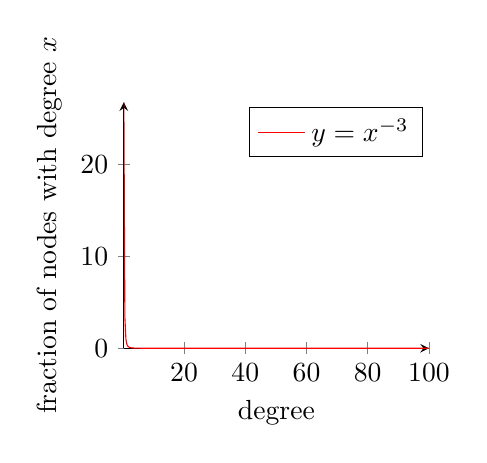
\begin{tikzpicture}
            \begin{axis}[
                width=0.45\textwidth,
                axis lines = left,
                xlabel = degree,
                ylabel = {fraction of nodes with degree $x$},
            ]
            \addplot [
                domain=0:100, 
                samples=300, 
                color=red,
            ]{1/(x^3)};
            \addlegendentry{$y=x^{-3}$}
            \end{axis}
        \end{tikzpicture}
        \hskip 7pt
        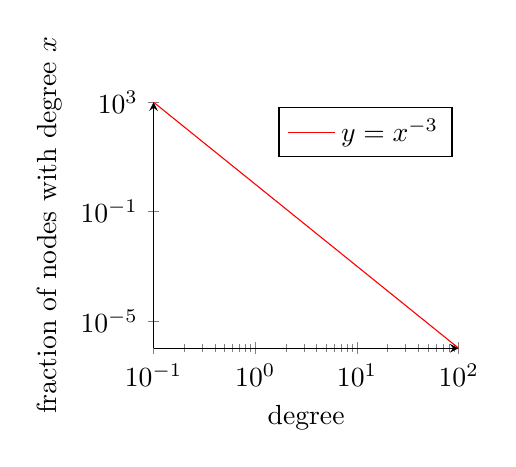
\begin{tikzpicture}
            \begin{axis}[
                width=0.45\textwidth,
                xmode=log,
                ymode=log,
                axis lines = left,
                xlabel = degree,
                ylabel = {fraction of nodes with degree $x$},
            ]
            \addplot [
                domain=0.1:100,
                samples=300,
                color=red,
            ]{1/(x^3)};
            \addlegendentry{$y=x^{-3}$}
            \end{axis}
        \end{tikzpicture}
        \caption{Power law distribution with linear and log log scale}
        \label{fig:power-law}
    \end{figure}
    